\documentclass[11pt]{article}
\usepackage{amsmath}
\usepackage{amssymb}
\usepackage{cite}
\usepackage{fancyhdr}
\usepackage{float}
\usepackage{geometry}
\usepackage{graphicx}
\usepackage{setspace}
\usepackage{subfigure}
\usepackage{times}
\usepackage{url}
\usepackage{multirow}
\usepackage{hyperref}
\usepackage{fontspec}
\usepackage[most]{tcolorbox}
\usepackage{xparse}
\usepackage{lipsum}
\usepackage{tikz}
\usepackage{quoting}
\usepackage{listings}
\usetikzlibrary{automata,positioning}

\usepackage{courier}
\lstset{basicstyle=\scriptsize \ttfamily,breaklines=true,mathescape=true}

\newcounter{example}
\def\exampletext{Example} % If English

\NewDocumentEnvironment{example}{ O{} }
{
	\colorlet{colexam}{red!55!black} % Global example color
	\newtcolorbox[use counter=example]{examplebox}{%
		% Example Frame Start
		empty,% Empty previously set parameters
		title={\exampletext: #1},% use \thetcbcounter to access the example counter text
		% Attaching a box requires an overlay
		attach boxed title to top left,
		% Ensures proper line breaking in longer titles
		minipage boxed title,
		% (boxed title style requires an overlay)
		boxed title style={empty,size=minimal,toprule=0pt,top=4pt,left=3mm,overlay={}},
		coltitle=colexam,fonttitle=\bfseries,
		before=\par\medskip\noindent,parbox=false,boxsep=0pt,left=3mm,right=0mm,top=2pt,breakable,pad at break=0mm,
		before upper=\csname @totalleftmargin\endcsname0pt, % Use instead of parbox=true. This ensures parskip is inherited by box.
		% Handles box when it exists on one page only
		overlay unbroken={\draw[colexam,line width=.5pt] ([xshift=-0pt]title.north west) -- ([xshift=-0pt]frame.south west); },
		% Handles multipage box: first page
		overlay first={\draw[colexam,line width=.5pt] ([xshift=-0pt]title.north west) -- ([xshift=-0pt]frame.south west); },
		% Handles multipage box: middle page
		overlay middle={\draw[colexam,line width=.5pt] ([xshift=-0pt]frame.north west) -- ([xshift=-0pt]frame.south west); },
		% Handles multipage box: last page
		overlay last={\draw[colexam,line width=.5pt] ([xshift=-0pt]frame.north west) -- ([xshift=-0pt]frame.south west); },%
	}
	\begin{examplebox}}
	{\end{examplebox}\endlist}






%\geometry{verbose,a4paper,
%          tmargin=2.5cm,bmargin=2.5cm,lmargin=2.5cm,rmargin=2.5cm}
\geometry{verbose,a4paper,
          tmargin=2.5cm,bmargin=2.5cm,lmargin=2.35cm,rmargin=2.35cm}

%\onehalfspacing
\setstretch{1.1}

%\DeclareGraphicsExtensions{.jpg,.pdf,.tif,.png,.tiff,.eps,.bb}

\newtheorem{definition}{Definition}
\newtheorem{problem}{Problem}

\pagestyle{fancy} \lhead{} \chead{} \rhead{Research proposal No.\
2714/19. PI\@: Gera Weiss} \lfoot{} \cfoot{} \rfoot{}
\renewcommand{\headrulewidth}{0pt}


\renewcommand{\thesection}{\Alph{section}.}
\renewcommand{\thesubsection}{\thesection\arabic{subsection}}

\renewcommand{\refname}{Bibliography}

{\makeatletter
 \gdef\xxxmark{%
   \expandafter\ifx\csname @mpargs\endcsname\relax % in minipage?
     \expandafter\ifx\csname @captype\endcsname\relax % in
%figure/caption?
       \marginpar{xxx}% not in a caption or minipage, can use marginpar
     \else
       xxx % notice trailing space
     \fi
   \else
     xxx % notice trailing space
   \fi}
 \gdef\xxx{\@ifnextchar[\xxx@lab\xxx@nolab}
 \long\gdef\xxx@lab[#1]#2{{\bf [\xxxmark #2 ---{\sc #1}]}}
 \long\gdef\xxx@nolab#1{{\bf [\xxxmark #1]}}
 % This turns them off:
 %\long\gdef\xxx@lab[#1]#2{}\long\gdef\xxx@nolab#1{}%
}
\def\ignore#1{}
%\newcommand{\sa}{SAF}
%\newcommand{\sasp}{SAF~~}


%\setstretch{1.1}




\begin{document}

\section*{Detailed description of the research program: \\Behavioural Composition of Hybrid Systems}


\section{Scientific Background}\label{sec:motivation}
The growth of cyber physical systems (CPS) such as embedded electronics, the internet of things (IoT), and advanced robotics is bringing information and control systems of increasing complexity to every aspects of our lives. This includes safety-critical systems, such as transportation systems (e.g., cars, aeroplanes, and trains), industrial plants and health care automation. Correct behaviour of such systems must be guaranteed under diverse environment conditions and potential failures; solutions have to meet cost, size, and power consumption requirements. This requires careful mathematical analysis and simulations of models of such systems. As many of these systems integrate continuous physical dynamics with discrete computations, we call them ``hybrid systems” and use models that integrate differential equations with automata and code to describe their dynamics.

There are different tools and languages that have been proposed over the years for describing hybrid (continuous and discrete) behaviours (or phenomena) in human-made systems and in nature. These languages are used in building descriptive models, simulators, and even final system code. Since the behaviours are often complex, the formal artefacts are often complex too, making them hard and expensive to create and to maintain, and susceptible to human error.

One way to tackle these issues, supported in most of the modelling techniques, is to formalise complex hybrid behaviours as a composition of simpler ones. However, all the composition techniques for hybrid systems that we are aware of allow for rich interactions only at discrete transitions while only basic tools for compositions of the continuous dynamics are available. In this proposal we bring evidence that composition according to the principles of scenario-based programming (SBP) can be particularly instrumental for breaking the description of complex systems as close as possible to the way stakeholders such as scientists, engineers, or high-school students perceive them. Based on these evidence, we propose to examine how SBP principles (those that we have today and future ones that we will develop along the research) can be used with several modelling languages and run-time implementations including MATLAB/Simulink diagrams and code, a combination of Python and SMT-solving language, and hybrid automata.We will study the technical capabilities and relative merits of the principles in general, and of each language, in terms of intuitiveness, executability, amenability to formal verification, alignment with textual natural language descriptions of the behaviours, and more. We believe that finding or creating languages in which such behavioural composition can be both precise and intuitive while enabling simulation, formal analysis and execution of final system code, can be extremely valuable in accelerating and simplifying the development and analysis of complex hybrid systems.


For completeness, we describe next the three  main scientific concepts around which this proposal is built:
\paragraph{Behavioural and scenario-based programming:} A widely accepted practice in software development is to formalise requirements in the form of use-cases and scenarios~\cite{Sutcliffe2003}. The programming approach termed behavioural programming (BP) extends this approach to using scenarios for the actual coding of software (executable specifications). Specifically, the method introduces scenario coding techniques and design approaches for constructing reactive systems~\cite{Harel1998} incrementally from their desired and undesired behaviours. The work on behavioural programming began with scenario-based programming, a way to create executable specifications of reactive systems, introduced through the language of live sequence charts (LSC) and its Play-Engine implementation~\cite{Damm2001,Marelly2002}. The initial purpose was to enable testing and refining specifications and prototypes, and the approach was later extended towards building actual systems. To this end, the underlying behavioural principles have also been implemented in imperative programming languages, via, e.g., the BPJ package~\cite{Harel2010} adding a more conventional programming point of view to that of requirement specification. Following this direction there are several tools supporting the behavioural programming principles in other languages such as Erlang~\cite{wiener2010coordinating}, C~\cite{katz2013module}  and with graphical tools such as the Play-Engine, PlayGo~\cite{Harel2010a}, and SBT~\cite{Greenyer2016}.

Our approach to scenario based specifications is based on the LSC language~\cite{Damm2001}. It allows GUI-based or natural-language-based playing in of behaviour scenarios, and is multi-modal, allowing constraints (for example, forbidden scenarios) to be part of the program. The approach has been generalised and extended also to other languages including Java, C++, Erlang, JavaScript and Blockly, and was termed behavioural programming (BP)~\cite{Harel2010}. Research results cover, among others, run-time look-ahead (smart playout)~\cite{Harel2002}, model-checking~\cite{Harel2011}, compositional verification~\cite{Harel2013}, synthesis~\cite{segall2011synthesis} and more.

\paragraph{Model Driven Engineering (MDE):} Model-driven engineering and software development~\cite{brambilla2017model,Shull2016} is geared to allow human stakeholders to develop and analyse a system using abstractions and formalism that are more closely aligned with their mental models than standard programming language code. MDE is supported by many languages, platforms and tools, including, among others, UML~\cite{UML2011} and SysML~\cite{OMGSysML2010}, AADL\cite{YANG2010}, MATLAB Simulink~\cite{Chaturvedi2017}, SCADE \cite{Sergent2012}, Ptolemy II~\cite{Hylands2003}, and Eclipse modelling Framework~\cite{BillMooreDavidDean2010}. The models, built in modelling languages, including domain-specific modelling languages and platforms, can be transformed into actual running code through automated model transformations. 

\paragraph{Hybrid Systems:}  Hybrid systems are dynamical systems that exhibit an interaction of continuous and discrete dynamics~\cite{Alur1995}. A prominent example are technological systems, called cyber physical systems (CPS), in which software based decision making and embedded control actions are combined with continuous, physical, processes~\cite{Lee2010}. Other examples include abstract description of physical, biological, and chemical systems in which quick dynamics are modeled as instantaneous~\cite{Lee2008}. To capture the dynamics of such systems, mathematical models are developed that combine the dynamics of the continuous parts of the system with the dynamics of discrete parts. These mathematical models come in different variations, all consisting of some form of differential or difference equations combined with automata or other discrete-event models~\cite{Lygeros2003}. The collection of analysis and synthesis techniques and the development of languages for these models forms the research and engineering area of hybrid systems, which plays a central role in many technological systems for which the analysis of the interconnections between the discrete and the continuous dynamics is needed.


\section{Research objectives \& expected significance}  
Languages and tools for modelling hybrid systems such as Simulink or Modelica are used in many industries including automotive, railway, aeronautics, energy, and more. The design of such systems is usually a concurrent activity involving different stakeholders (engineers, teams or companies). They cooperate by separating concerns, where using different formalism and models of computation describing different aspects of the continuous and of the discrete dynamics. The process usually starts  from a set of high-level functional and non-functional requirements and aim at producing heterogeneous executable models, resulting from the composition of several domain-specific models that describe different concerns on the system.
Currently all concerns are usually captured in a uniform modelling and simulation environment with a fixed semantics of the relationships between the various models. In this area, Simulink is a de facto standard design framework, and other tools such as Modelica follow the modelling approach. However, more and more domain-specific modelling languages recently appeared for levering on specific experience of particular domains such as embedded and real-time systems. For pure discrete systems, Model Driven Engineering and behavioural Programming provide facilities to design and implement new languages and composition techniques for combining the orthogonal concerns, usually discrete, of a system [10,28]. However, the current state of these facilities suffer from being disconnected from continuous modelling and simulation environments of physical dynamics.
In this work, we propose to explore the relationship between different components of hybrid systems. The main objective is to study the power of behavioural interfaces for rich composition between models that describe different aspects of the dynamics of a system, both at the level of event composition and at the level of composition of the continuous flows between the events.
We aim at providing a modelling workbench where users can easily define aspects of behaviours and use them to model discrete and continuous dynamics of a hybrid system. The workbench would offer advanced mechanisms for testing and for debugging the system. The composition semantics will allow for maximal flexibility in separating the concerns as the stakeholders see fit. It will not force modellers to discuss discrete and continuous dynamics in isolation and it will not force them to integrate only by discrete events.


\section{Detailed description of the proposed research}
We will develop a modelling approach for hybrid dynamical systems based on an adaptation of the behavioural programming (BP) model proposed in [6]. Specifically, the proposed model will be an extension of BP with tools to support scenario based modelling of hybrid systems where time evolves both discretely and continuously and the state contains real valued vectors.

The behavioural programming (BP) modelling approach was designed for modelling and for programming discrete reactive systems. A BP model consists of a specification of a set of components, called b-threads, each of which is a program that runs concurrently and pauses when it wants to synchronise with the other b-threads (by invoking a method called bp.sync). When all b-threads are at a synchronisation point, the b-threads communicate via a simple protocol that allows them to coordinate an event or to wait for an external event. When an event is chosen or when an external event arrives, the process continues by resuming all the b-threads that wait for the event and waiting for them to reach a synchronisation point again.
The standard approach for modelling hybrid systems mathematically is by hybrid automata, a finite state machine with continuous variables whose evolution is described by differential equations. 

In this work we propose an alternative approach for modelling hybrid dynamical systems. The main design goal for the modelling approach proposed here is the ability of breaking compound specifications into independent model modules (b-threads), each of which representing a separate aspect of the behaviour. This goal, of course, is common to other approaches. For example, Newton's laws of motion that describe the relationship between the motion of a body and the forces acting upon it, are an example of explaining a complex behaviour based on a simple composition of a set of relatively simple components. Another example, is the composition of hybrid automata where each component is a hybrid automaton and the components coordinate a joint behaviour using shared variables and events~\cite{DBLP:conf/hybrid/WeissA07}. The modelling approach we present in this work aims at providing more refined mechanisms for interactions between the components of the model, allowing for models whose components are better aligned with the aspects of the behaviours as people perceive them, as demonstrated by the examples we provide. 

We demonstrate the proposed modelling approach using two proof-of-concept software tools. One is based on the well known MATLAB/Simulink (\url{www.mathworks.com/help/simulink}) modelling language and the other is based on the Z3 SMT (\url{github.com/Z3Prover/z3}) solver  with its interface to the Python programming language (\url{ericpony.github.io/z3py-tutorial}). These two tools are very different in nature, but they both demonstrate a common modelling approach, as follows. Each behavioural aspect of the system is modeled by the host language (Simulink or Python) with direct idioms for synchronising with the other components and for posting logical constraints over the evolving state of the system. The constraints consist of ``request" and ``block" conditions, i.e., each component can specify what may happen and what cannot happen. Each joint decision is an assignment to a set of discrete and real-valued variables that marks a step in a simulation of the modeled dynamical system. The b-threads are informed of the decision (assignment) and the process goes on repeatedly.	

To demonstrate this, let us start with a very simple example of a bouncing ball, as described, e.g., in \url{en.wikipedia.org/wiki/Hybrid_system}. The ball, considered as a point mass, is dropped and bounces when it hits the ground, losing energy with each bounce. This system can be modeled by one b-thread that tells the story of the direction that changes when the ball hits the ground, one b-thread that models the constant gravitational force, and one b-thread that models the energy that decreases when hitting the ground. See the details of this example in Section 3 below. The difference between our description of this system and the hybrid-automaton models such as the one  described in KeYmaera [31]  and the one described on the Wikipedia page mentioned above is that our modelling approach does not bind us to describing a complete differential equation or a full account of the transition relation --- we allow modelling each aspect of the behaviour separately and the differential equations and the transitions between emerge implicitly. This is demonstrated in our preliminary results below.

\subsection{Working hypothesis}

Our working hypothesis is that composition techniques based on behavioural programming idioms will perform better than current modelling and composition techniques for hybrid systems in terms of allowing better alignment to the aspects of the system that stakeholders perceive and better maintenance and debugging procedures.

\subsection{Research design \& methods}
Our modelling approach is inspired by a cinematic effect used in science-fiction movies such as ``The Matrix''~\url{en.wikipedia.org/wiki/The_Matrix}, called ``bullet time", where the dynamics of the world are suspended or frozen, and the characters can take time to reflect upon, and react to, the situation. Analogously, our model consists of agents, termed \emph{b-threads}, that follow the evolution of the state and can instantaneously make recommendations that help direct it. Formally, we propose to model the state space of the system as  $\mathcal{X} \subseteq \mathbb{R}^n$ and the state at any given time $t$ as a variable $x \in \mathcal{X}$. The state $x$ evolves both continuously over time, or via a `jump', also termed \emph{reset}. The changes in the state are subject to 
declarations that  the b-threads make about forces that operate on the objects in the system and in the environment, optional actions that  the system can take and constraints over those actions . 

Each  b-thread, $b \in \mathcal{BT}$, is an observer of the state that specifies at any moment $t$, possibly based on the current state $x$, the sets $may(b,x,t) \subseteq \mathcal{X}$ and $must(b,x,t) \subseteq \mathcal{X}$  representing, respectively,  requested and blocked vectors. The evolution begins in a specified set of possible initial states $X_0 \subseteq X$ and is governed  by the differential inclusion:
\begin{equation}
\dot{x} \in \bigcup_{b \in \mathcal{BT}} may(b,x,t) \cap  \bigcap_{b \in \mathcal{BT}} must(b,x,t). 
\label{eq:diffeqn}
\end{equation}
where $\dot{x}$ is the derivative of $x$ with respect to time. To allow for modelling hybrid phenomena, each b-thread,  $b \in \mathcal{BT}$, can also specify an additional pair of sets  $may_{rst}(b,x,t) \subseteq \mathcal{X}$ and $must_{rst}(b,x,t) \subseteq \mathcal{X}$  and if the set 

$$rst=\bigcup_{b \in \mathcal{BT}} mayReset(b,x,t) \cap   \bigcap_{b \in \mathcal{BT}} mustReset(b,x,t) $$is not empty, then the state may reset instantaneously to a state in this set. Note that we are not bounding the time between two resets, i.e., a sequence of resets may be triggered in an instance and in ever shrinking intervals. This, of course, allows for Zeno behaviours that may have useful interpretations in different application domains. Note also that the model is not deterministic --- it allows for multiple discrete and continuous evolution. Again, the interpretation of nondeterminism in a model depends on the application domain. 

While the b-threads are formally functions that map the current state and the elapsed time to the four four sets described above, we propose in this paper several languages for describing these functions using graphical and intuitive textual formats. Before we dive into the details of how we propose to model the b-threads, consider the following example, designed to demonstrate the power of the proposed composition mechanism, in which the b-threads are modeled directly as pure functions. 

\begin{example}[Colliding particles (borrowed from~\cite{goebel2009hybrid})]
	\label{ex:collison}
Consider two particles that move toward each other, collide, and then move away from each other on a one dimensional line. The state of this system can be modeled as a vector $x = (p, v) = ((p_1, p_2),(v_1, v_2))$, where $p_1$ and $p_2$ denote the particles’ positions and $v_1$ and $v_2$ denote the particles’ velocities.  The dynamics of the system is modeled by the following b-threads:
	\begin{itemize}
		\item $b_1$: Relation between position and velocities: $may(b_1,x,t)=\{ \dot{x}\colon \dot{p}=v\}$.
		\item $b_2$: Newton's first law: $may(b_2,x,t)=\{ \dot{x} \colon \dot{v}=0\}$. 
		\item $b_3$: Conservation of momentum: 
		$$must(b_3,x,t)=mustReset(b_3,x,t)=\{ x^+\colon m_1 v_1^+ + m_2 v_2^+ =  m_1 v_1 + m_2 v_2 \}$$
		where $m_1$ and $m_2$ are constants modelling the masses of the particles. 
		\item $b_4$: Energy dissipation and direction reversal on hit: $$mayReset(b_4,x,t)=
		\begin{cases}
		\emptyset & \text{if }p_1 \neq p_2; \\
		\{ x^+\colon v_1^+ - v_2^+ =  - \rho (v_1 - v_2) \} & \text{if }p_1 =  p_2;
		\end{cases}
		$$ where $\rho \in (0,1)$ is a constant modelling a restitution coefficient. 
	\end{itemize}
	All the $may$ sets not mentioned above are assumed to be empty and all the $must$ sets not mentioned are assumed to be $\mathcal{X}$.
\end{example}

Comparing the model proposed in the above example to the model described in~\cite{goebel2009hybrid} for the same system shows how our modelling approach allows for better decomposition of the aspects of a behaviour. Specifically,  $b_1$ and $b_2$ are modeled together in~\cite{goebel2009hybrid} and so are $b_3$ and $b_4$. Since each of these aspects is usually conceived separately by engineers and scientists, even in the text of~\cite{goebel2009hybrid}, we argue that this kind of separation, allowed by our approach, can be useful for improving engineering and scientific methodologies. 

\subsection{Preliminary results}
In this section we outline some initial experiments we ran with different tools to demonstrate the possibilities that the new modelling approach allows:

\subsubsection{A discretization based implementation of hybrid models}
\label{sec:simulation}  
Many useful tools for designing analysing continuous and hybrid models use simulation based on time discretization. Specifically, in this paper we propose, as one of the alternative modelling languages, an extension to hybrid-systems of tools we have developed for modelling discrete-time reactive systems. The  extension is based on interpreting traces generated by a discrete-time behavioural system as traces of a continuous-time model as described below.

The core of the interpretation is viewing sequences of states (trace) as discretizations of continuous signals. To allow this, we assume that the discrete system that generated the traces satisfies the following properties:
\begin{enumerate}
	\item There is a parameter set $\Gamma$ and a bijection that maps any $(\gamma, \delta) \in \Gamma \times (0,\infty)$ to a trace  $s_{\gamma,\delta}(1),s_{\gamma,\delta}(2),\dots$ of the system and vice verse. 
	\item Each state $s_{\gamma,\delta}(k)$ contains the $n$ dimensional vectors $x_{\gamma,\delta}(k)$ and $x_{\gamma,\delta}'(k)$ and a non-negative number $d_{\gamma,\delta}(k)$  such that $0 \leq d_{\gamma,\delta}(k) \leq \delta$.
	\item If $d_{\gamma,\delta}(k) \neq 0$ then  $x_{\gamma,\delta}(k+1) - x_{\gamma,\delta}(k) = x'_{\gamma,\delta}(k) \cdot d_{\gamma,\delta}(k)$.
	\item  For any $t>0$ and $\gamma \in \Gamma$,  $\lim_{\delta \to 0} x_{\gamma,\delta}(\lfloor\frac{t}{\Delta}\rfloor)$ converges to a vector in $\mathbb{R}^n$ that we call $x_\gamma(t)$.
\end{enumerate}

Under these assumptions, we say that the discrete system models the set of piecewise continuous signals $\{ x_\gamma \colon \gamma \in \Gamma \}$.  With this convention, discrete systems can be used to model behavioural hybrid models, as demonstrated by the following example:

\begin{example}[Using discretization for modelling simple continuous dynamics]
	\label{ex:sin}
	For a parameter set $\Gamma = (0,\infty)\times (0,\infty)$, consider a discrete behavioural-programming system where the b-threads are parametrized by a pair $(\omega,\varphi) \in \Gamma$ and a number $\delta >0$ as follows:
	\begin{itemize}
		\item A ``Direction" b-thread always requests that $x_{\gamma,\delta}'(k) = \cos(\omega\delta k + \varphi)$ and blocks assignments of $x'_{\gamma,\delta}(k)$ with any other value.
		\item A ``Fixed Step" b-thread always requests that $d_{\gamma,\delta}(k) = \delta$ and and blocks  assignments of $d_{\gamma,\delta}(k)$ with any other value.
		\item A ``Derivative" b-thread always requests that $x_{\gamma,\delta}(k+1) = x_{\gamma,\delta}(k) +  {x}'_{\gamma,\delta}(k)\cdot  d_{\gamma,\delta}(k)$ and blocks assignments of $x_{\gamma,\delta}(k)$ with any other value.
	\end{itemize}
	Consider also the  behavioural hybrid model consisting of a single b-threads $b$ that starts with choosing $\omega$ and $\varphi$ nondeterministically and then issues the time-dependent $must(b,x,t)=may(b,x,t)=\{  \cos(\omega t + \varphi )\}$. Note that the sets of executions of both systems are the same. Because the "Direction" b-thread is very similar to the (only) b-thread in the behavioural hybrid model, and because the  other two b-threads are generic, not specific to this example, we say that the "Direction" b-thread is an implementation of the behavioural hybrid model.
\end{example}

\subsubsection{A MATLAB/Simulink based tool}
\label{sec:simulink}
In this section we describe a prototype BP modelling tool we have developed based on the well-known MATLAB/Simulink modelling tool. With our tool the b-threads can be written using common Simulink blocks, the standard language of Simulink models, so it is natural for Simulink developers to understand and adopt the tool. We tried Two simulation cases, the first is of a one-dimensional bouncing ball, shown below, and the second is of a two-dimensional path tracking robot. I both cases the model came clear and easy to understand (as confirmed by fellow engineers and collaborators).

The continuous BP engine, ESM (Event Selection Mechanism), is implemented using a dedicated S-function block. Its inputs are the b-threads Request/Block/Reset (RBR) statements as strings converted to vectors. The ESM evaluate these strings and uses the request/block statements as inputs for the MATLAB Symbolic Math solver. The solver outputs all the possible events to choose from. Then a selection is made, using random or specific user defined optimisation selection process.   

\begin{figure}[ht]
	\centering
	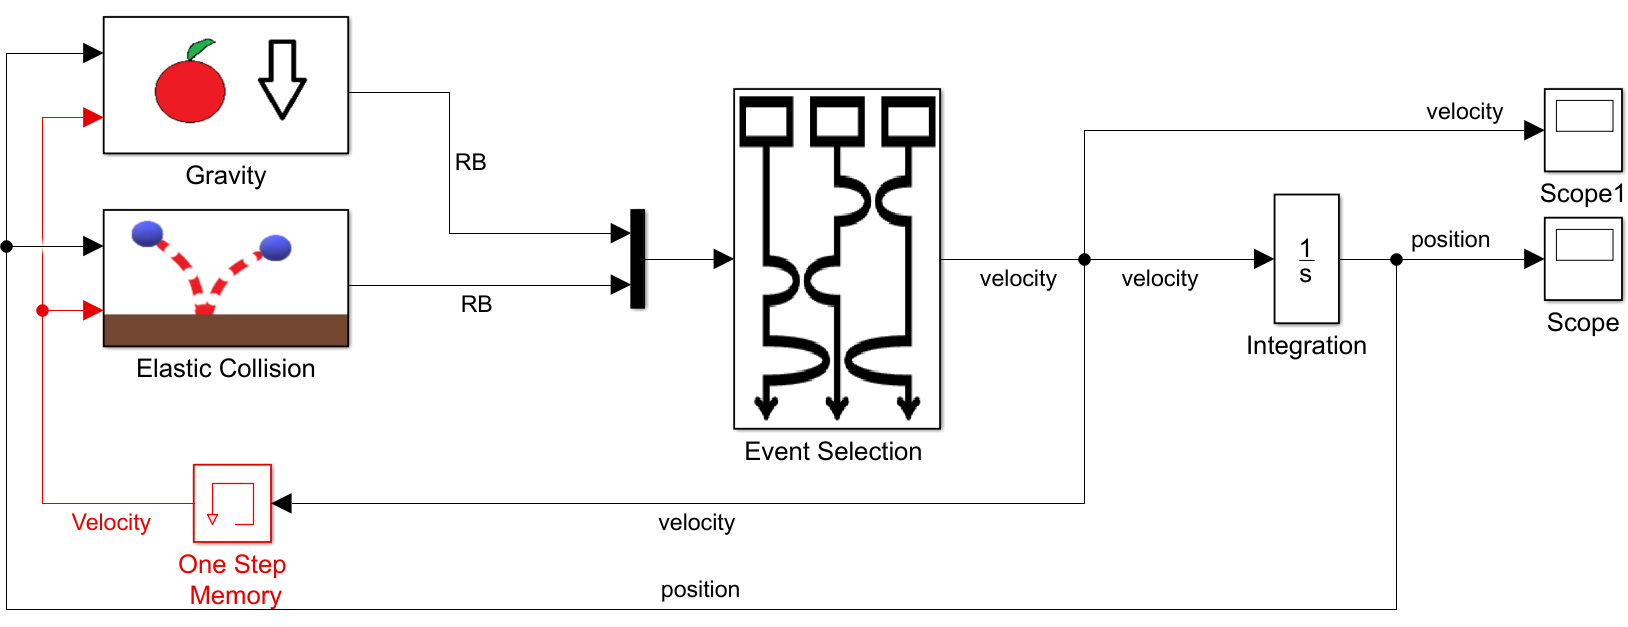
\includegraphics[width=\columnwidth]{ODBB.png}
	\caption{Simulink model of the one dimensional bouncing ball. Similar to the python code described below and the automata based model, we see that it it possible to weave two independent b-threads, each modelling a separated aspect of the behaviour using an application agnostic event selection and integration mechanism.}
	\label{fig:bouncing ball}
\end{figure}

\subsubsection{A Z3/Python based tool}
\label{sec:Z3}

A second tool we have developed to demonstrate the composition mechanisms proposed in this paper is based on the Pyhton programming language and the Z3 theorem prover. The tool is extension of the behavioural programming paradigm as implemented. e.g., in the BPjs library~\cite{Ashrov2015}. The extension is developed  in two steps: (1) We present a discrete-time execution mechanism where b-threads specify ``must" and ``may" logical constraints instead of event sets; (2) We use this mechanism together with the discretization based semantics discussed in Section~\ref{sec:simulation}.

We apply the Z3 solver for interpreting and for solving the ``may'' and ``must'' constraints that the b-threads specify. Each b-thread is implemented as a Python generator that yields a Python dictionary that may contain any subsets of the keys ``may'', ``must'', and ``wait-for''. Each such key is associated with a Z3 constraint. The execution mechanism, whose code is given in Listing~\ref{code:execution}, takes care of running the b-threads by asking them to go to their next yield, collecting the dictionaries that each b-thread yields (called ``bids'' in the code), and finding a model that satisfies all the constraints using the Z3 solver. This goes in a loop until no such model is found. In each round of the loop only the b-threads that waited for the chosen model (their `wait-for' constraint is satisfied) are moved to their next yield, the other b-threads stay still and their bids are maintained. 

With this mechanism, for example, one can specify the following b-threads:
\begin{lstlisting}[caption={A simple example of a program that uses the solver based execution mechanism.},captionpos=b,frame = single]
hot = Bool('hot')
cold = Bool('cold')

def three_hot():
	for i in range(3):
		yield {'may': hot, 'wait-for': hot}


def three_cold():
	for i in range(3):
		yield {'may': cold, 'wait-for': cold}


def no_two_hot_in_a_row():
	while True:
		yield {'wait-for': hot}
		yield {'must': Not(hot), 'wait-for': Not(hot)}


def logger():
	t = 0
	while True:
		yield {'wait-for': true}
		print(">>>> %d: %s" % (t, m))
		t = t + 1 
\end{lstlisting}

\begin{lstlisting}[caption={The output of the above program.},captionpos=b,frame = single]
>>>> 0: [cold = False, hot = True]
>>>> 1: [hot = False, cold = True]
>>>> 2: [cold = False, hot = True]
>>>> 3: [hot = False, cold = True]
>>>> 4: [cold = False, hot = True]
>>>> 5: [hot = False, cold = True]
\end{lstlisting}

The above, of course, is a general mechanism that does not target only hybrid systems. It can, however, serve as a tool for modelling hybrid systems as follows. We propose to add a b-thread that takes care of time increment and of approximating an integration of variables with respect to their derivative: 

\begin{lstlisting}[caption={A b-thread that specifies that the `dot' version of each variable is its derivative using a simple linear approximation.},captionpos=b,frame = single]
def dot():
	global t
	while True:
		yield {
			'must': Or(reset, And(var1 == (m[$var_1$] + (m[$var_1$dot] * deltaT)),
							$\vdots$                $\vdots$ 
			                      varn == (m[$var_n$] + (m[$var_n$dot] * deltaT)),
	
			'wait-for': true}
	
		if (not is_true(m[reset])):
			t = t + deltaT            
\end{lstlisting}

This code assumes that our system consists of a a Boolean variable called \lstinline{reset} and a set of pairs of real-valued variables \lstinline{$var_1$},\lstinline{$var_1$dot},\dots,\lstinline{$var_n$},\lstinline{$var_n$dot}. The Python variable \lstinline{m} is the model that the solver produces in each execution round. The Python variable \lstinline{t} is the time passed since the beginning of the simulation. The b-thread simply says that if the state does not reset, it must progress such that the each variable is an integration of its derivative with respect to time.

% Add the firefly model here?

\subsubsection{Hybrid Automata based Models}
\label{sec:hybrid-automata}
The improvement we seek in this paper, when compared to the existing work on hybrid automata is in allowing better control of the structure of a model. Specifically, we subscribe to the principle that guided the development of C++:

\begin{quoting}
	``It should provide facilities for organising programs into well-defined separate parts, and provide facilities for combining separately developed parts.'' (Bjarne Stroustrup~\cite{Stroustrup07})
\end{quoting} 

Similar to the relation between \lstinline{C} and \lstinline{C++}, the relation of hybrid behavioural models and hybrid automata is that the former add tools for modularity and for abstraction. Since we are proposing a new language for integrating hybrid models, our method can also be used as an extension to time-automata, as discussed below.

When modelling natural phenomena, modularity is particularly useful as a tool that allows for explicit separation of the scientific principles that the model encapsulates. Consider, for example, the simple hybrid automaton describing a bouncing ball depicted in Figure~\ref{fig:ha-bouncingball}. To demonstrate the alternative modelling technique proposed in this paper, imagine a group of school students studying this system. They may first notice that the ball goes up and down and write the b-thread listed as \lstinline{updown}. In this model, $x$ denotes the displacement (height) of the ball and $s$ denotes its speed (a positive scalar). Next, they may notice that the speed of the ball is decreased by some factor $\gamma \in (0,1)$ when it hits the floor and formulate the b-thread listed as \lstinline{bounce}. Then, to complete the model, they may make some speed measurements and add a third b-thread, shown as \lstinline{gravity}, that models the gravitational acceleration. We are not saying that this is the only way to model this system, nor that it is better in all aspects. Our only claim is that the freedom that our modelling approach allows gives tools to build a model whose components are aligned with the students view of the phenomena that they are studying.

\begin{figure}[H]
	\begin{center}
		\label{fig:ha-bouncingball}
		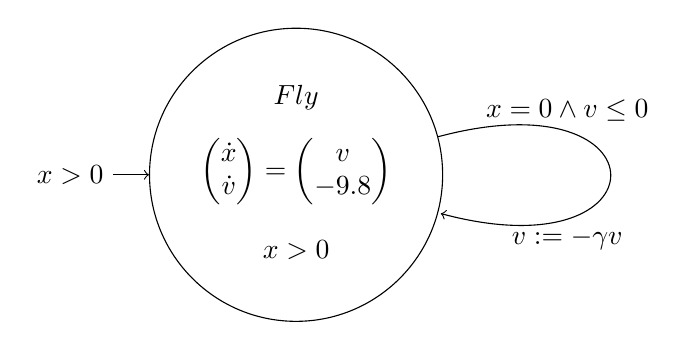
\begin{tikzpicture}[initial text = $x>0$] 
		\node[state,initial] (q_0)   
		{$\begin{matrix}
			Fly \\[0.3cm] 
			\begin{pmatrix}\dot{x} \\ \dot{v}\end{pmatrix}=\begin{pmatrix}v \\ -9.8\end{pmatrix} \\[0.6cm] 
			x > 0
			\end{matrix}$ }; 
		\path[->] 
		(q_0)  edge [loop right] 
		node [above,near start] {$x = 0 \wedge v \leq 0$} 
		node [below, near end] {$v := -\gamma v$} 
		(); 
		
		\end{tikzpicture}
	\end{center}
	\caption{A standard hybrid-automata model of a bouncing ball of weight $1$Kg. The variable $x$ represents the displacement (height0 of the ball, the variable $v$ represents its velocity, and the constant $\gamma \in (0,1)$ models the fraction of speed preserved when hitting the ground.}
\end{figure}

\begin{lstlisting}[caption={B-Threads for the bouncing ball example.  \lstinline{updown} models that, repeatedly in a loop, the speed increases while the ball goes down and then it decreases while the ball goes up, \lstinline{bounce} model that a fraction of the speed is lost with every bounce, and \lstinline{gravity} models the acceleration.},captionpos=b,frame = single]
def updown():
    while True:
        yield {'may': And(xdot == -s, sdot > 0), 
               'wait-for': x <= 0}

        yield {'may': And(xdot == s, sdot < 0), 
               'wait-for': s <= 0}

def bounce():
    while True:
    
        yield {'wait-for': x <= 0}
        
        yield {'must': And(reset, s == m[s] * 0.8),
               'wait-for': true}
        
        yield {'wait-for': x > 0}
    
def gravity():
    yield {'must': Or(sdot == 9.8, sdot == -9.8)}
\end{lstlisting}


Note that the three aspects that we were able to describe separately with  a behavioural hybrid model must be combined together when describing the system with a hybrid automaton. This may not be a major issue when dealing with simple systems, but it may be a significant factor with more complex systems.

Hybrid automata can be used to model the individual b-threads in a behavioural hybrid model, as demonstrated in Figure~3. Note that this approach does not directly allows for a b-thread that changes its request or block sets continuously,  as we do, for example, in the example in Section~\ref{ex:sin} above. To allow this we can have the request be based on a continuously varying variable as shown in Figure~4.  



\begin{figure}[H]
	\begin{center}
		\label{fig:ha-b-threads-bouncingball}
		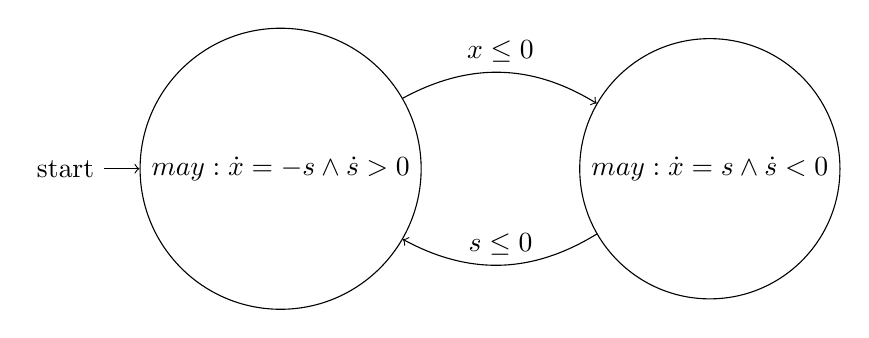
\begin{tikzpicture}
		\node[state,initial] (q_0)   
		{$\begin{matrix}
		    may: \dot{x} = -s \wedge \dot{s}>0
			\end{matrix}$ }; 

		\node[state, right=2cm of q_0] (q_1)   
		{$\begin{matrix}
		    may: \dot{x} = s \wedge \dot{s}< 0
			\end{matrix}$ }; 
			
			
		\path[->] 
		(q_0)  edge  [bend left]
		node [above] {$x \leq 0$} 
		(q_1); 

		\path[->] 
		(q_1)  edge [bend left]
		node [above] {$s \leq 0$} 
		(q_0); 

		
		\end{tikzpicture}
	\end{center}
	\caption{The first b-thread in of the bouncing ball example modelled using an extended time-automaton where each mode can specify $may$ and $must$ constraints.}
\end{figure}

\begin{figure}[H]
    \label{fig:ha-b-threads-sin}
	\begin{center}
		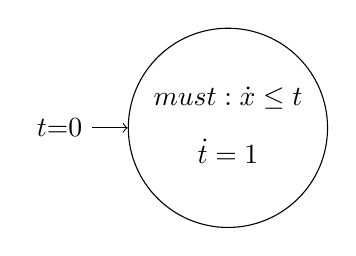
\begin{tikzpicture}[initial text = $t{=}0$] 
		\node[state,initial] (q_0)   
		{$\begin{matrix}
  			must: \dot{x} \leq t \\[0.3cm] 
  			\dot{t} = 1
  		  \end{matrix}$ };  
	\end{tikzpicture}
	\end{center}
	\caption{A simple b-thread that enforces a continuously growing upper bound on $\dot{x}$. This demonstrates that we can combine internal dynamics of the hybrid automaton with the $may$ and $must$ constraints to obtain full flexibility.}
\end{figure}

Existing work on composition of hybrid automata such as~\cite{SHIFT} focus on interactions at discrete transitions. Our work allows for more advanced interactions where components can complement each other both on the  discrete and on the continuous level, as demonstrated by the above example. 



\subsubsection{Code for the event selection mechanism}
For the purpose of developing this proposal, we have implemented a new event selection mechanism in Python as shown in Listing~\ref{code:execution}. This is a generalised behavioural programming protocol that applies the Z3 solver and Python generators to allow for b-threads that specify constraints rather than sets of events, as we do in other behavioural programming implementations. In the context of the proposed project, we will enrol Ph.D. and M.Sc. students for developing such mechanism and specialise them for the specific challenge of bringing improved tools for modelling hybrid systems. We expect that this effort will also contribute to other applications of behavioural programming. Already in the development of the proposal, we have learned much from experiencing with the new mechanism and from modelling example systems with it.



\begin{lstlisting}[label={code:execution},caption={An execution mechanism that runs a set of b-threads, each specified as a Python generator that yields a list of dictionaries with `may', `must', and `wait-for' constraints.},captionpos=b,frame = single]
def run(bthreads):
    bids = []
    
    # Run all bthreads to their initial yield
    for bt in bthreads:
   
    # Get the bid that the b-thread yielded
    bid = next(bt)
    
    # Add areference of the b-thread to the bid
    bid['bt'] = bt
    
    # Append the biod to the list of bids
    bids.append(bid)
    
    # Main loop
    while True:
        may, must = (False, True)
    
    # Collect the `may' and `must' constraints
    for bid in bids:
        if 'may' in bid:
            may = Or(may, bid['may'])
    
        if 'must' in bid:
            must = And(must, bid['must'])
    
    # Compute a model that satisfies all the `must' constraints and at least one `may' 
    sl = Solver()
    sl.add(And(may, must))
    
    if sl.check() == sat:
        m = sl.model()
    else:
        print("--- End of the super-step ---")
        break
    
    # Advance the threads
    newbids = []
    for bid in bids:
        # If the bid has a `wait-for' key and the constraint associated with it is satisfied
        if 'wait-for' in bid and is_true(m.eval(bid['wait-for'])):
            # Advance the b-thread to its next yield and get its new bid
            nb = next(bid['bt'], 'Finished')
            
        if not nb == 'Finished':
            # Add a ref. the b-thread to the bid
            nb['bt'] = bid['bt']
            
            # Add it the list of new-bids
            newbids.append(nb)
        else:
            # Add the old bid to the list of new bids
            newbids.append(bid)
    
    # Switch to the new bids list
    bids = newbids
\end{lstlisting}



\subsection{Conditions and facilities available for the researcher for performing the research}

The PI is an expert in both behavioural programming and in hybrid systems. The main condition needed for the research is excellent research students and collaborators that can challenge new ideas, propose case-studies, and examine new technologies and theories. We are lucky to have many such students at the department of computer science at the Ben Gurion University coming from diverse background including computer science, software engineering, mechanical engineering, electrical engineering, and more. The PI is also lucky to have collaborators in all these departments and in other universities. 

In addition, the PI, with his students, developed in recent years an advanced robotics laboratory focused on studying control theoretic and software engineering aspects of flying drones. The laboratory is equipped with different types of quadrotors, an advanced array of cameras for tracking the location of the drones, and other equipment needed for academic research in this field.

We are also currently developing a new laboratory for research and teaching of space software. This laboratory consists of a state-of-the-art nano-satellite platform connected to an advanced simulation environment that allows us to develop and test production-quality software for satellites. This project aims at showing that behavioural programming can handle the full complexity of a real system and offers measurable advantages.

We will use the above laboratories and other research projects by collaborators (smart buildings, robotic agriculture, biological modelling, etc.) to examine the methods that we will develop in the propose research and to challenge their effectiveness. 

\subsection{Expected results; pitfalls; alternatives in case of failure}
	
We expect this project to result with new modelling techniques for hybrid systems. The main new type of features that we will develop is new mechanisms for integrating sub-models applying new integration semantics. As demonstrated by the preliminary work described above, we believe that this can allow for new methodologies, new analysis tools, and new algorithms that support more efficient of accurate hybrid models.

We will run case-studies and user-studies to examine how the tools that we develop perform in real-world scenarios. This studies may not show perfect result in the first run, in which case we will study the pitfalls, improve the tools, and try again.

\bibliographystyle{plain}
\bibliography{references,mend}

\end{document}

